\documentclass{beamer}
\usepackage{geometry}
\usepackage[english]{babel}
\usepackage[utf8]{inputenc}
\usepackage{amsmath}
\usepackage{amsfonts}
\usepackage{amssymb}
\usepackage{tikz}
\usetikzlibrary{quotes, angles}
\usepackage{graphicx}

%\usepackage{pgfplots}
%\pgfplotsset{width=10cm,compat=1.9}
%\usepackage{pgfplotstable}

\setlength{\headheight}{26pt}%doesn't seem to fix warning

\usepackage{fancyhdr}
\pagestyle{fancy}
\fancyhf{}

%\rhead{\small{13 November 2018}}
\lhead{\small{BECA / Dr. Huson / Geometry Unit 4}}

\renewcommand{\headrulewidth}{0pt}

\title{Mathematics Class Slides}
\subtitle{Bronx Early College Academy}
\author{Chris Huson}
\date{26 November 2018}

\begin{document}
\frame{\titlepage}
\section[Outline]{}
\frame{\tableofcontents}


\section{4.1 Project: Triangle congruence project, Monday 26 November}
  \frame
  {
    \frametitle{Construction project: Triangle congruence}
    \framesubtitle{CCSS: HSG.CO.C.9 Prove geometric theorems \hspace{\stretch{1}} \alert{4.1}}

    \begin{block}{Four pages of $\triangle$ duplication constructions for binder}
    \begin{enumerate}
        \item Side-side-side (SSS)
        \item Side-angle-side (SAS)
        \item Angle-side-angle (ASA)
        \item Side-side-angle (SSA), false, ``ambiguous case"
    \end{enumerate}
        Grading criteria (20 points)
    \begin{enumerate}
        \item Complete and correct construction
        \item State postulate or theorem. (written steps not necessary)
        \item MLA header, center title \& last name on right
        \item Precise, elegant, mathematical aesthetic
    \end{enumerate}
    \end{block}
    Due Friday November 30
    }

\section{4.1 Drui: Triangle congruence. Monday 26 November}
  \frame
  {
    \frametitle{GQ: How do we construct congruent triangles?}
    \framesubtitle{CCSS: HSG.CO.C.9 Prove geometric theorems \hspace{\stretch{1}} \alert{4.1 Monday 26 November}}

    \begin{block}{Do Now: }
      \begin{enumerate}
        \item Trig review problems handout
        \item $+, \triangle$ What is working? What would you change?
      \end{enumerate}
    \end{block}
    Seating chart \\
    2nd trimester norms and expectations \\
    $\triangle$ congruence construction project, SSS\\
    Homework packet review, trig problems \\[0.5cm]
    Homework: Distance, midpoint, and slope review, handout\\
    \alert{Parent-teacher conferences Thursday \& Friday}
  }


\section{4.2 Drui: Deltamath. Tuesday 27 November}
  \frame
  {
    \frametitle{GQ: How do we use trigonometric ratios?}
    \framesubtitle{CCSS: HSG.CO.D.12 Congruence, geometric constructions \hspace{\stretch{1}} \alert{4.2 Tuesday 27 November}}

    \begin{block}{Do Now: SAS $\triangle$ congruence}
    \begin{enumerate}
        \item Duplicate a side, duplicate an angle, duplicate a side.
        \item Angle must be the \emph{included} angle, between the two sides
        \item $\triangle ABC \cong \triangle A'B'C'$ iff $\overline{AB} \cong \overline{A'B'}, \angle A \cong \angle A', \text{ and } \overline{AC} \cong \overline{A'C'}$
    \end{enumerate}
    \end{block}
    Geogegra intro (?)\\
    Deltamath assessment: distance, midpoint, and slope\\
    Deltamath homework: trig ratios, triangle relationships\\[0.5cm]
    Homework: Complete deltamath (10pm deadline)\\
    \alert{Parent-teacher conferences Thursday \& Friday}
  }


\section{4.3 Drui: Triangle proofs. Wednesday 28 November}
  \frame
  {
    \frametitle{GQ: How do we prove triangles congruent?}
    \framesubtitle{CCSS: HSG.CO.D.12 Congruence, geometric constructions \hspace{\stretch{1}} \alert{4.3 Wednesday 28 November}}
    Do Now: Theorems review handout \\
    Triangle sum, transversal, vertical
    \begin{block}{Angle-side-angle (ASA) $\triangle$ congruence}
    \begin{enumerate}
        \item Duplicate an angle, duplicate a side, duplicate an angle
        \item $\triangle ABC \cong \triangle A'B'C'$ iff $\angle A \cong \angle A', \overline{AB} \cong \overline{A'B'}, \text{ and } \angle B \cong \angle B'$
    \end{enumerate}
    \end{block}
    Lesson: \\
    Triangle congruence proofs\\
    Assessment: distance, midpoint, and slope\\[0.5cm]
    Homework: Pretest packet. \alert{Test Friday}
  }

\section{4.4 Drui: Pretest review. Thursday 29 November}
  \frame
  {
    \frametitle{GQ: How do we prove triangles congruent?}
    \framesubtitle{CCSS: HSG.CO.D.12 Congruence, geometric constructions \hspace{\stretch{1}} \alert{4.4 Thursday 29 November}}

    Do Now: Triangle congruence practice handout

    \begin{block}{SSA $\triangle$ congruence (or ASS, ``jack ass theorem")}
    \begin{enumerate}
        \item Duplicate an angle, duplicate a side, duplicate an side
        \item Given $\triangle ABC$ if $ \angle A \cong \angle A', \overline{AB} \cong \overline{A'B'}, \text{ and } \overline{BC} \cong \overline{B'C'}$ then two possible $\triangle$s may result.
    \end{enumerate}
    \end{block}
    Lesson: \\
    Review problems for take home test\\[0.5cm]
    Homework: Complete $\triangle \cong$ project \alert{due tomorrow}
  }

\section{4.5 Drui: Exam. Friday 30 November}
  \frame
  {
    \frametitle{GQ: How do we prove triangles congruent?}
    \framesubtitle{CCSS: HSG.CO.D.12 Congruence, geometric constructions \hspace{\stretch{1}} \alert{4.5 Friday 30 November}}

    \begin{block}{Review for unit exam}
    \end{block}
    Triangle congruence project due\\[0.5cm]
    Homework: Take home test
  }

  \section{4.6 Drui: Translations Monday December 3}
    \frame
    {
      \frametitle{GQ: How do we translate the plane?}
      \framesubtitle{CCSS: HSG.CO.D.12 Congruence, geometric constructions \hspace{\stretch{1}} \alert{4.6 Monday December 3}}

      %\begin{block}{Unit exam}
      %\end{block}
      Transformations, translations\\
      Hexagon (\& square) construction project due Friday\\[0.5cm]
      Homework: Hexagon construction
    }

  \section{4.7 Deltamath Translations Tuesday December 4}
    \frame
    {
      \frametitle{GQ: How do we translate the plane?}
      \framesubtitle{CCSS: HSG.CO.D.12 Congruence, geometric constructions \hspace{\stretch{1}} \alert{4.7 Tuesday December 4}}

      \begin{block}{HL Triangle congruence}
      \end{block}
      Deltamath classwork: Transformations, translations, hexagon construction\\[0.5cm]
      Homework: Deltamath homework package
    }

  \section{4.8 Drui: Translations Wednesday December 5}
    \frame
    {
      \frametitle{GQ: How do we translate the plane?}
      \framesubtitle{CCSS: HSG.CO.D.12 Congruence, geometric constructions \hspace{\stretch{1}} \alert{4.8 Wednesday December 5}}

      \begin{block}{Triangle congruence handout. Problem \#1 \\ Spicy: keep going!}
        Hint: use theorems from transversals and parallel lines
      \end{block} \vspace{0.5cm}
      Triangle congruence proofs\\
      Square construction\\
      Rigid motion, pre-image$\rightarrow$image, compositions. pp. 545-550\\[0.5cm]
      Homework: Congruence handout
    }

  \section{4.9 Drui: Reflections Thursday December 6}
    \frame
    {
      \frametitle{GQ: How do we reflect objects on the plane?}
      \framesubtitle{CCSS: HSG.CO.D.12 Congruence, geometric constructions \hspace{\stretch{1}} \alert{4.9 Thursday December 6}}

      \begin{block}{Triangle congruence, translation handout.}
        %Hint: use theorems from transversals and parallel lines
      \end{block} \vspace{0.5cm}
      Constructing the line of reflection given pre-image$\rightarrow$image\\
      Reflection across a line, orientation. pp. 554-557\\[0.5cm]
      Homework: Congruence handout
    }

  \section{4.10 Drui: Rotation Friday December 7}
    \frame
    {
      \frametitle{GQ: How do we rotate objects on the plane?}
      \framesubtitle{CCSS: HSG.CO.D.12 Congruence, geometric constructions \hspace{\stretch{1}} \alert{4.10 Friday December 7}}

      \begin{block}{Triangle congruence, transformation handout.}
        %Hint: use theorems from transversals and parallel lines
      \end{block} \vspace{0.5cm}
      Center and angle of rotation mapping pre-image$\rightarrow$image\\
      pp. 561-567\\[0.5cm]
      Homework: Congruence, transformation handout
    }

  \section{4.11 Drui: Rounding, volume formulas Monday December 10}
    \frame
    {
      \frametitle{GQ: What are the arithmetic skills in geometry?}
      \framesubtitle{CCSS: HSG.CO.D.12 Congruence, geometric constructions \hspace{\stretch{1}} \alert{4.11 Monday December 10}}

      \begin{block}{Do Now: Answer on a separate sheet of paper to turn in.}
        Triangle $A'B'C'$ is the image of triangle $ABC$ after a translation of 2 units to the right and 3 units up. Is triangle $ABC$ congruent to triangle $A'B'C'$? Explain why.
      \end{block} \vspace{0.5cm}
      Lesson: Rounding, volume calculations using the formula sheet\\[0.5cm]
      \alert{Test Thursday} \\[0.5cm]
      Homework: Pretest handout, due Wednesday
    }

  \section{4.11 Rigid motion: Transformations that maintain length and angle measures Monday December 10}
    \frame
    {
      \frametitle{Rigid motion}
      \framesubtitle{When does a transformations maintain length and angle measures?}

      Triangle $A'B'C'$ is the image of triangle $ABC$ after a translation of 2 units to the right and 3 units up. Is triangle $ABC$ congruent to triangle $A'B'C'$ ? Explain why.\\[0.25cm]

      \pause \includegraphics[width=0.9\textwidth]{isometry_JN2018-25-sol.png}\\
      \pause \includegraphics[width=0.9\textwidth]{isometry_JN2018-25-sol2.png}
    }

  \section{4.11 Symmetry: objects invariant under a transformation Monday December 10}
    \frame
    {
      \frametitle{Symmetry}
      \framesubtitle{When is an object unchanged by a transformation?}

      If when an object $A \rightarrow A'$ and $A = A'$ then we say it is symmetric. \\
      Reflection: \emph{axis of symmetry}\\
      Rotation: \emph{center and angle of rotation}\\[0.25cm]
      Example: Regular polygons are symmetrical\\[0.25cm]

      \pause 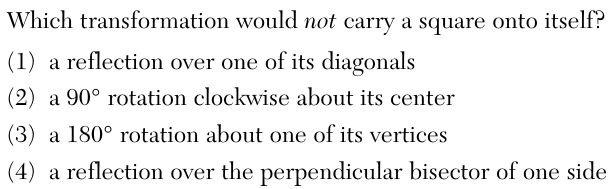
\includegraphics[width=0.7\textwidth]{symmetry-square_JA2018-15.png}\\
      \pause 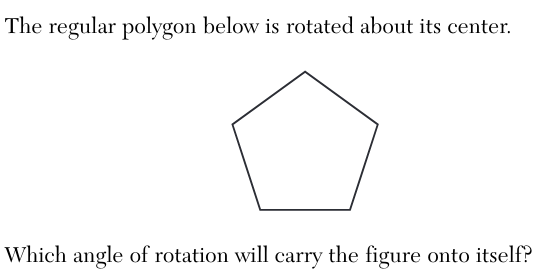
\includegraphics[width=0.7\textwidth]{symmetry_JN2018-19.png}
    }

  \section{4.12 Deltamath Translations Tuesday December 11}
    \frame
    {
      \frametitle{GQ: How do we translate the plane?}
      \framesubtitle{CCSS: HSG.CO.D.12 Congruence, geometric constructions \hspace{\stretch{1}} \alert{4.12 Tuesday December 11}}

      \begin{block}{Area formulas: triangle, semi-circle}
      \end{block}
      Deltamath classwork: Transformations, volume calculations\\[0.5cm]
      \alert{Test Thursday} \\[0.5cm]
      Homework: Deltamath homework package
    }

  \section{4.13 Drui: Radians, symmetry; Test review Wednesday December 12}
    \frame
    {
      \frametitle{GQ: How do we convert angle measure units?}
      \framesubtitle{CCSS: HSG.CO.D.12 Congruence, geometric constructions \hspace{\stretch{1}} \alert{4.13 Wednesday December 12}}

      \begin{block}{Triangle congruence, transformation handout.}
        %Hint: use theorems from transversals and parallel lines
      \end{block} \vspace{0.5cm}
      Lesson: radians to degrees formulas, symmetry\\
      Review for test\\[0.5cm]
      Intensives daily homework protocol \\[0.5cm]
      Homework: Study for \alert{Test Tomorrow}
    }

  \section{4.14 Drui: Dilation Thursday December 13}
    \frame
    {
      \frametitle{GQ: How do we translate objects on the plane?}
      \framesubtitle{CCSS: HSG.CO.D.12 Congruence, geometric constructions \hspace{\stretch{1}} \alert{4.14 Thursday December 13}}

      \begin{block}{\centering Test}
        %Hint: use theorems from transversals and parallel lines
      \end{block} \vspace{0.5cm}
      %Review for test\\[0.5cm]
      Homework: Review packet, due Monday Room 450\\[0.5cm]
      (Intensives daily homework)
    }

  \section{4.15 Deltamath Review Friday December 14}
    \frame
    {
      \frametitle{GQ: How do we translate the plane?}
      \framesubtitle{CCSS: HSG.CO.D.12 Congruence, geometric constructions \hspace{\stretch{1}} \alert{4.15 Friday December 14}}

      \begin{block}{Intensives daily homework protocol}
      \end{block}
      Deltamath classwork: Holiday review\\[0.5cm]
      Homework: Deltamath homework package
    }


  \section{X.1 Drui: Dilation Monday January 7}
    \frame
    {
      \frametitle{GQ: How do we dilate objects on the plane?}
      \framesubtitle{CCSS: HSG.CO.D.12 Congruence, geometric constructions \hspace{\stretch{1}} \alert{4.11 Monday December 10}}

      \begin{block}{Triangle congruence, transformation handout.}
        %Hint: use theorems from transversals and parallel lines
      \end{block} \vspace{0.5cm}
      Center of dilation and scale factor mapping pre-image$\rightarrow$image\\
      pp. 587-591\\[0.5cm]
      Homework:
    }

\end{document}
